
\section{Deliverable 6: Swiss roll}


\begin{solve}    

\begin{figure}[H]
    \centering
    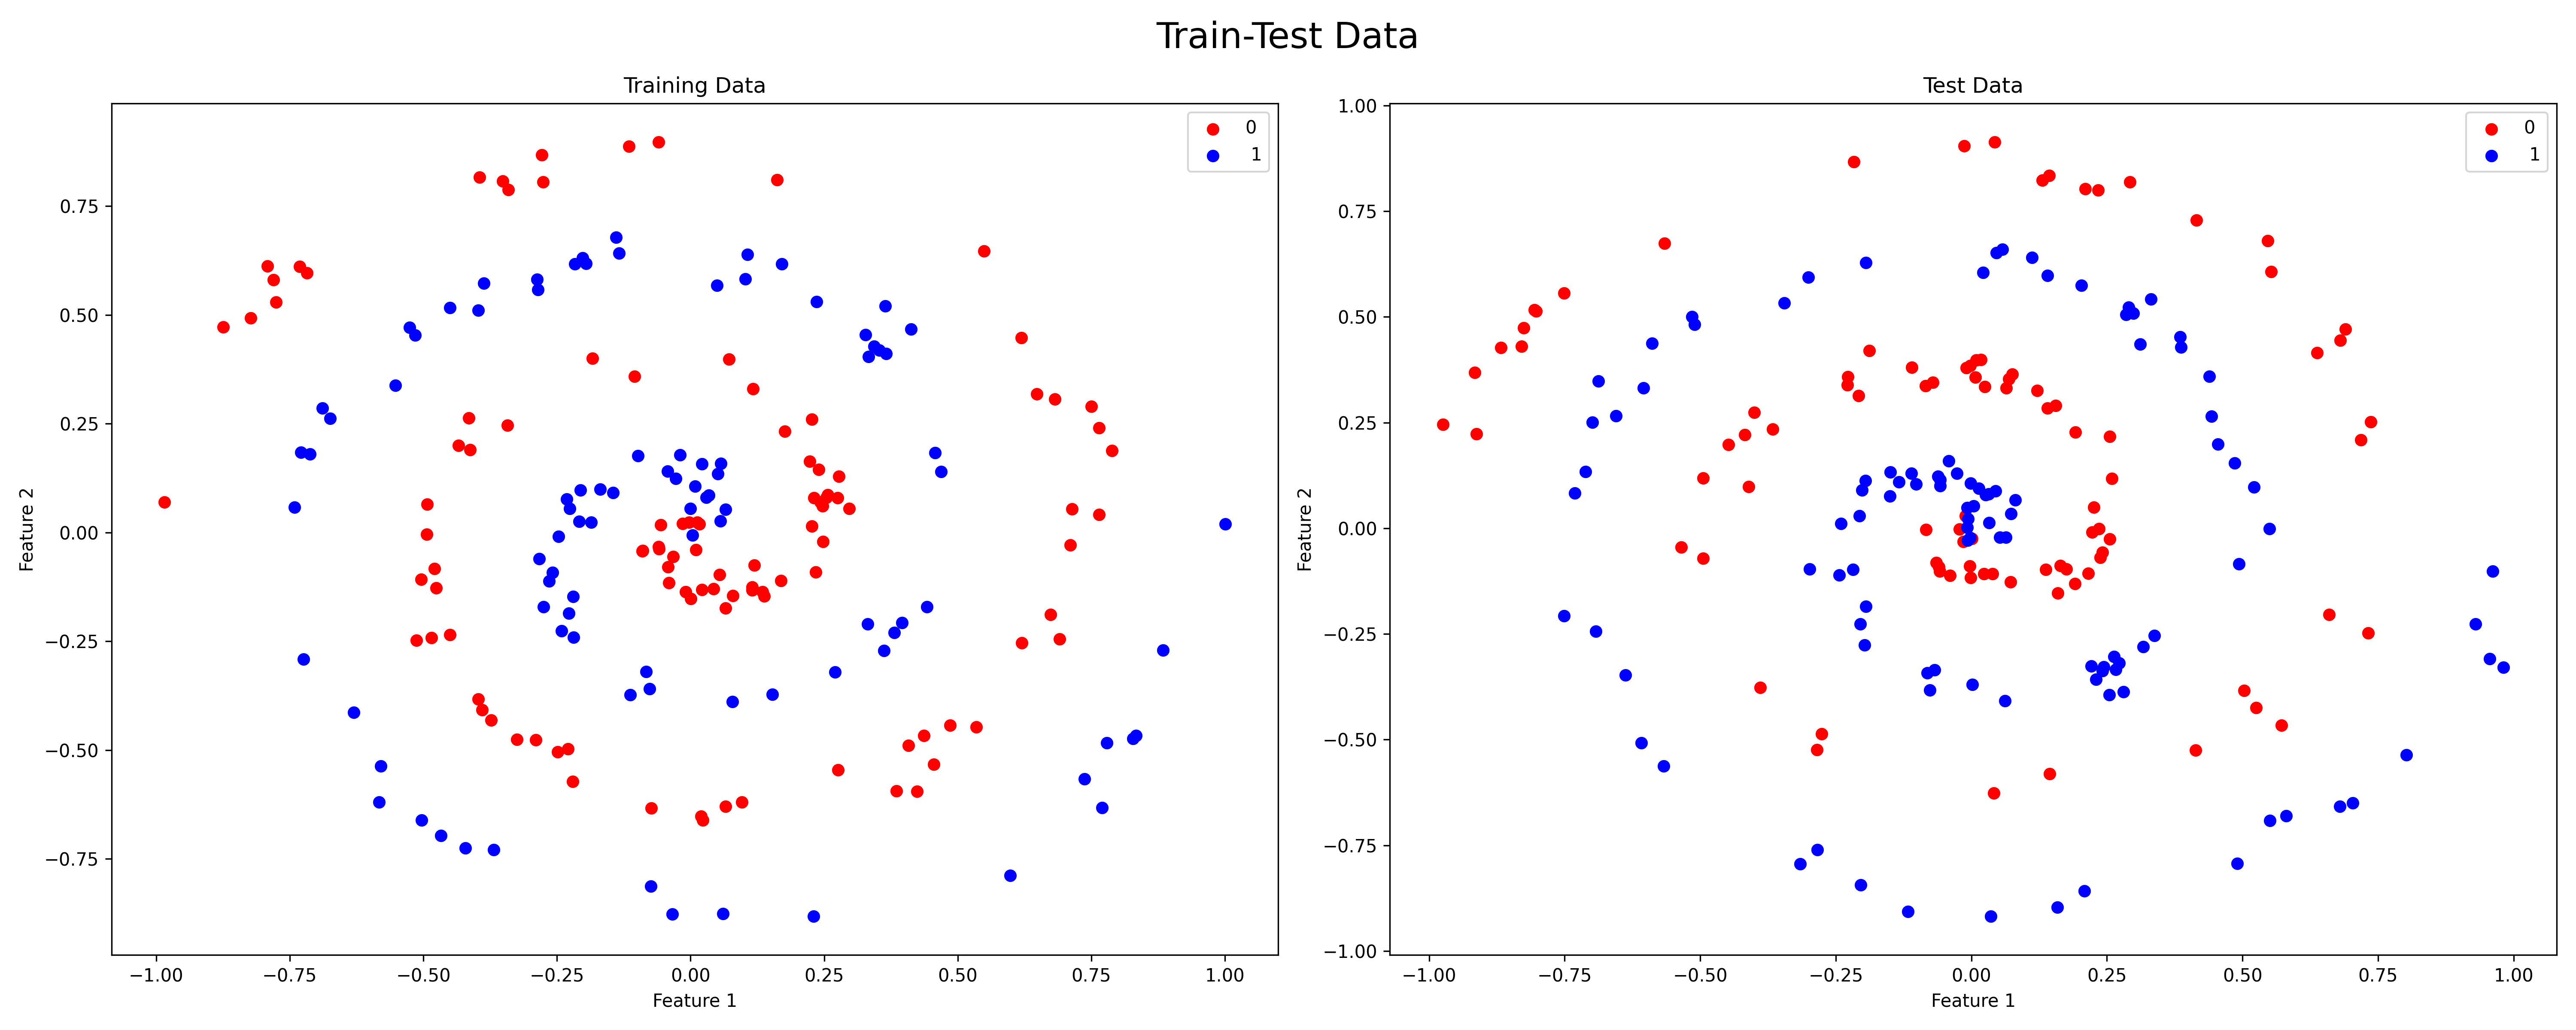
\includegraphics[width=0.7\textwidth]{plots/6_train_test_swiss-roll.png}
    \caption{Swiss-Roll dataset (train, test set with 200 points each)}
\end{figure}


\begin{lstlisting}[language=python]
dim_in, dim_out = x_train.shape[1], 2
hidden_neuron_list = [8, 16, 64, 12]
activation_list = ['ReLU','ReLU', 'ReLU','ReLU','LinearActivation']
opt_init = 'xavier'
opt_loss = CrossEntropyLoss()
mlp = MLP(dim_in, dim_out, hidden_neuron_list, activation_list, opt_init)
opt_optim = Adam(mlp, learning_rate=0.01)
print(mlp.summary())
    
-----------------------------------------------------------------
Model Summary
-------------
Layer 1: Linear - A Dim: 2, Output Dim: 8, Parameters: 24
Layer 2: ReLU
Layer 3: Linear - A Dim: 8, Output Dim: 16, Parameters: 144
Layer 4: ReLU
Layer 5: Linear - A Dim: 16, Output Dim: 64, Parameters: 1088
Layer 6: ReLU
Layer 7: Linear - A Dim: 64, Output Dim: 12, Parameters: 780
Layer 8: ReLU
Layer 9: Linear - A Dim: 12, Output Dim: 2, Parameters: 26
Layer 10: LinearActivation
Total Parameters: 2062
\end{lstlisting}

\begin{figure}[H]
    \centering
    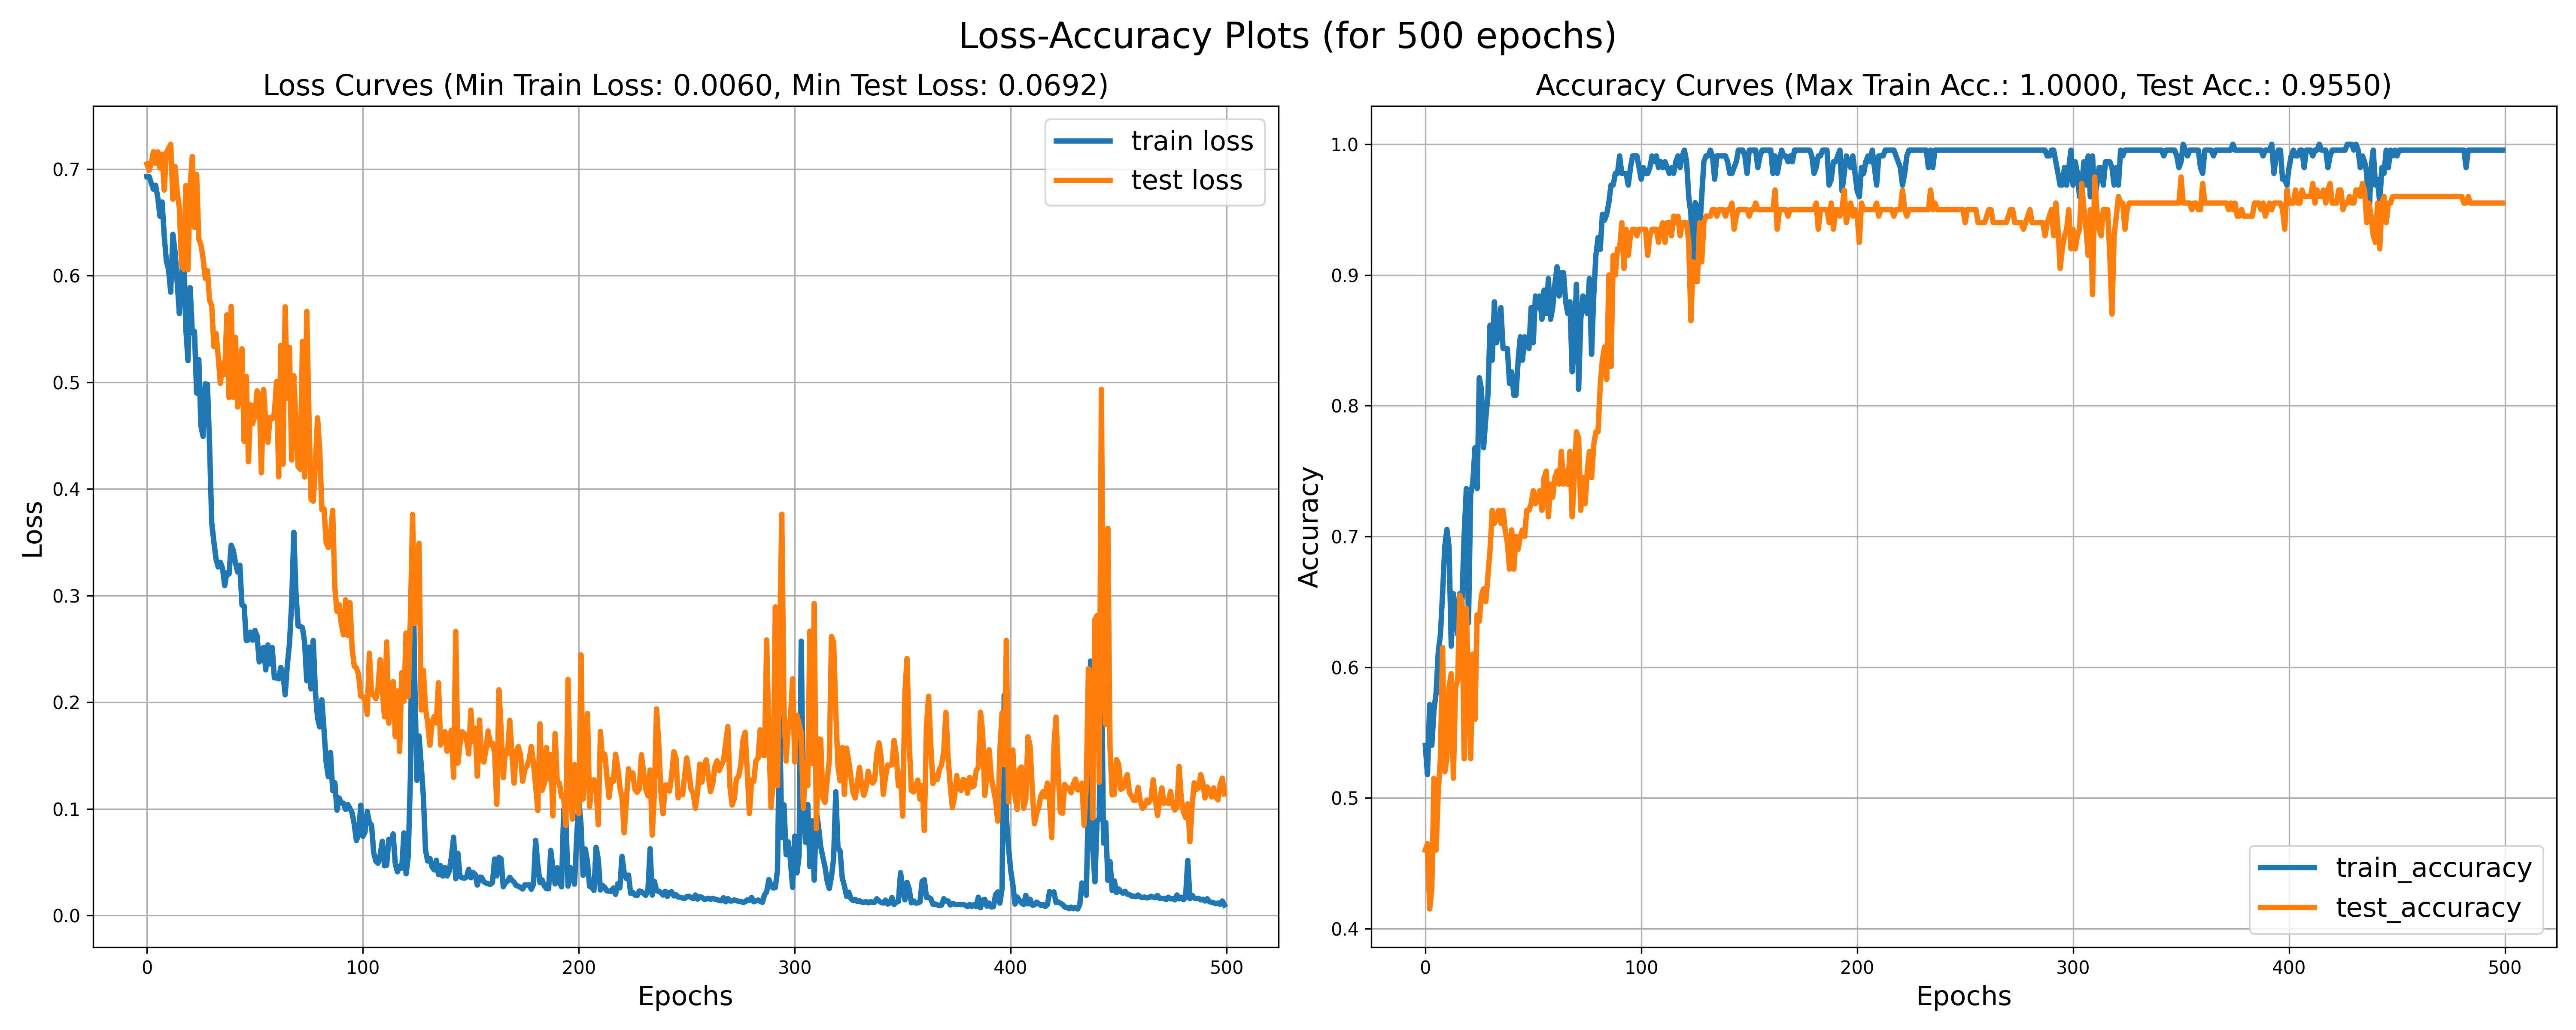
\includegraphics[width=0.9\textwidth]{plots/6_spiral_adam_more_layersloss_acc.png}
    \caption{Loss and accuracy for Swiss-roll dataset (train, test set with 200 points each), Adam optimizer (lr = .01), 500 epochs, Cost function: CrossEntropyLoss, Xaiver initialization}
    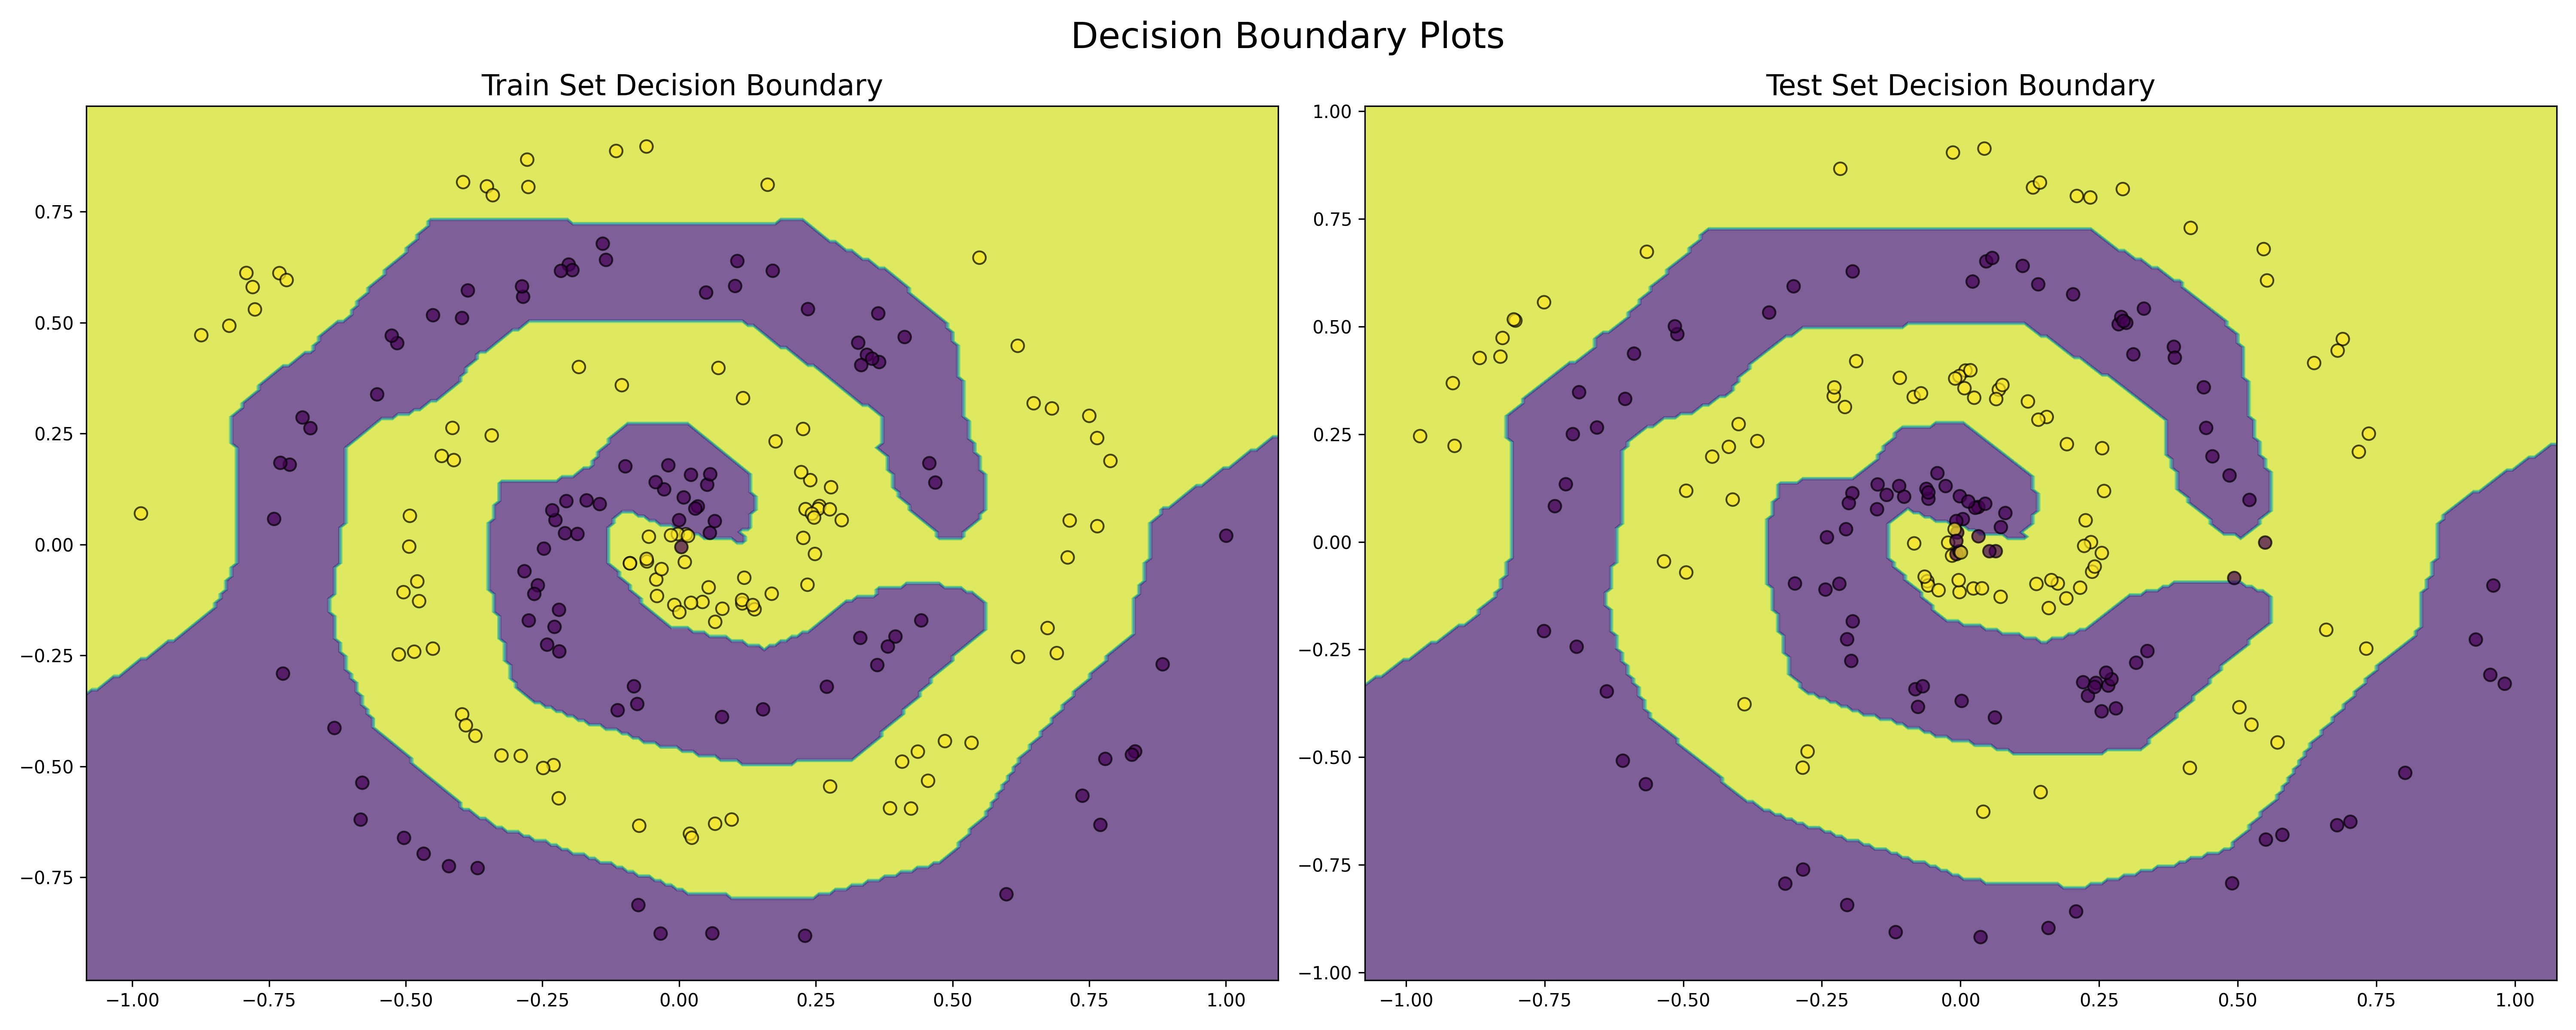
\includegraphics[width=0.8\textwidth]{plots/6_spiral_adam_more_layersboundary.png}
    \caption{(L2Loss) Decision boundary for Swiss-Roll separable dataset (train, test set with 200 points each)}
\end{figure}

% ############################################

\end{solve}
